%---------------------------------------------------------------------------------------------------
% Analysis
%---------------------------------------------------------------------------------------------------
\newpage
\chapter{Requirement Analysis}
 The main requirement of this thesis is to design, and implement an Archive service i.e. back-end web service for the MARS framework. The service's role is to
 archive the MARS resources mentioned in Subsection \ref{subsection:MARSResource} from the Ceph cluster \cite{Ceph} to the 
 NAS\footnote{NAS: Network Attached Storage} Synology drive \cite{Synology}.

 This service targets any user who desires to archive the MARS resources needed for a simulation including the existing simulation results, which would
 be analyzed in the future. The Archive service would expose its API, calling it, one can archive and restore the resources. The exposed
 API can be later integrated in the MARS graphical interface (MARS Teaching User Interface). The MARS Teaching API acts as proxy between the users 
 and the MARS back-end Microservices, as it provides some level of abstraction by hiding unnecessary endpoints for the user in the graphical interface.

 Figure \ref{fig:archiveUseCase} presents the use case of the system with its expected behavior. The main intention of the diagram is to show the
 general description which actions possible using this service. As seen from the diagram, a user is associated with three use cases i.e. archive, restore,
 and getting the job status. 
 While Archiving it is noticed that the project is marked first, this is done because this locks the resources for other services if they want to make any changes.
 
 The requirements for the thesis are divided into three different categories non-functional, 
 functional and technical aspects. 
 \begin{figure}[H]
    \centering 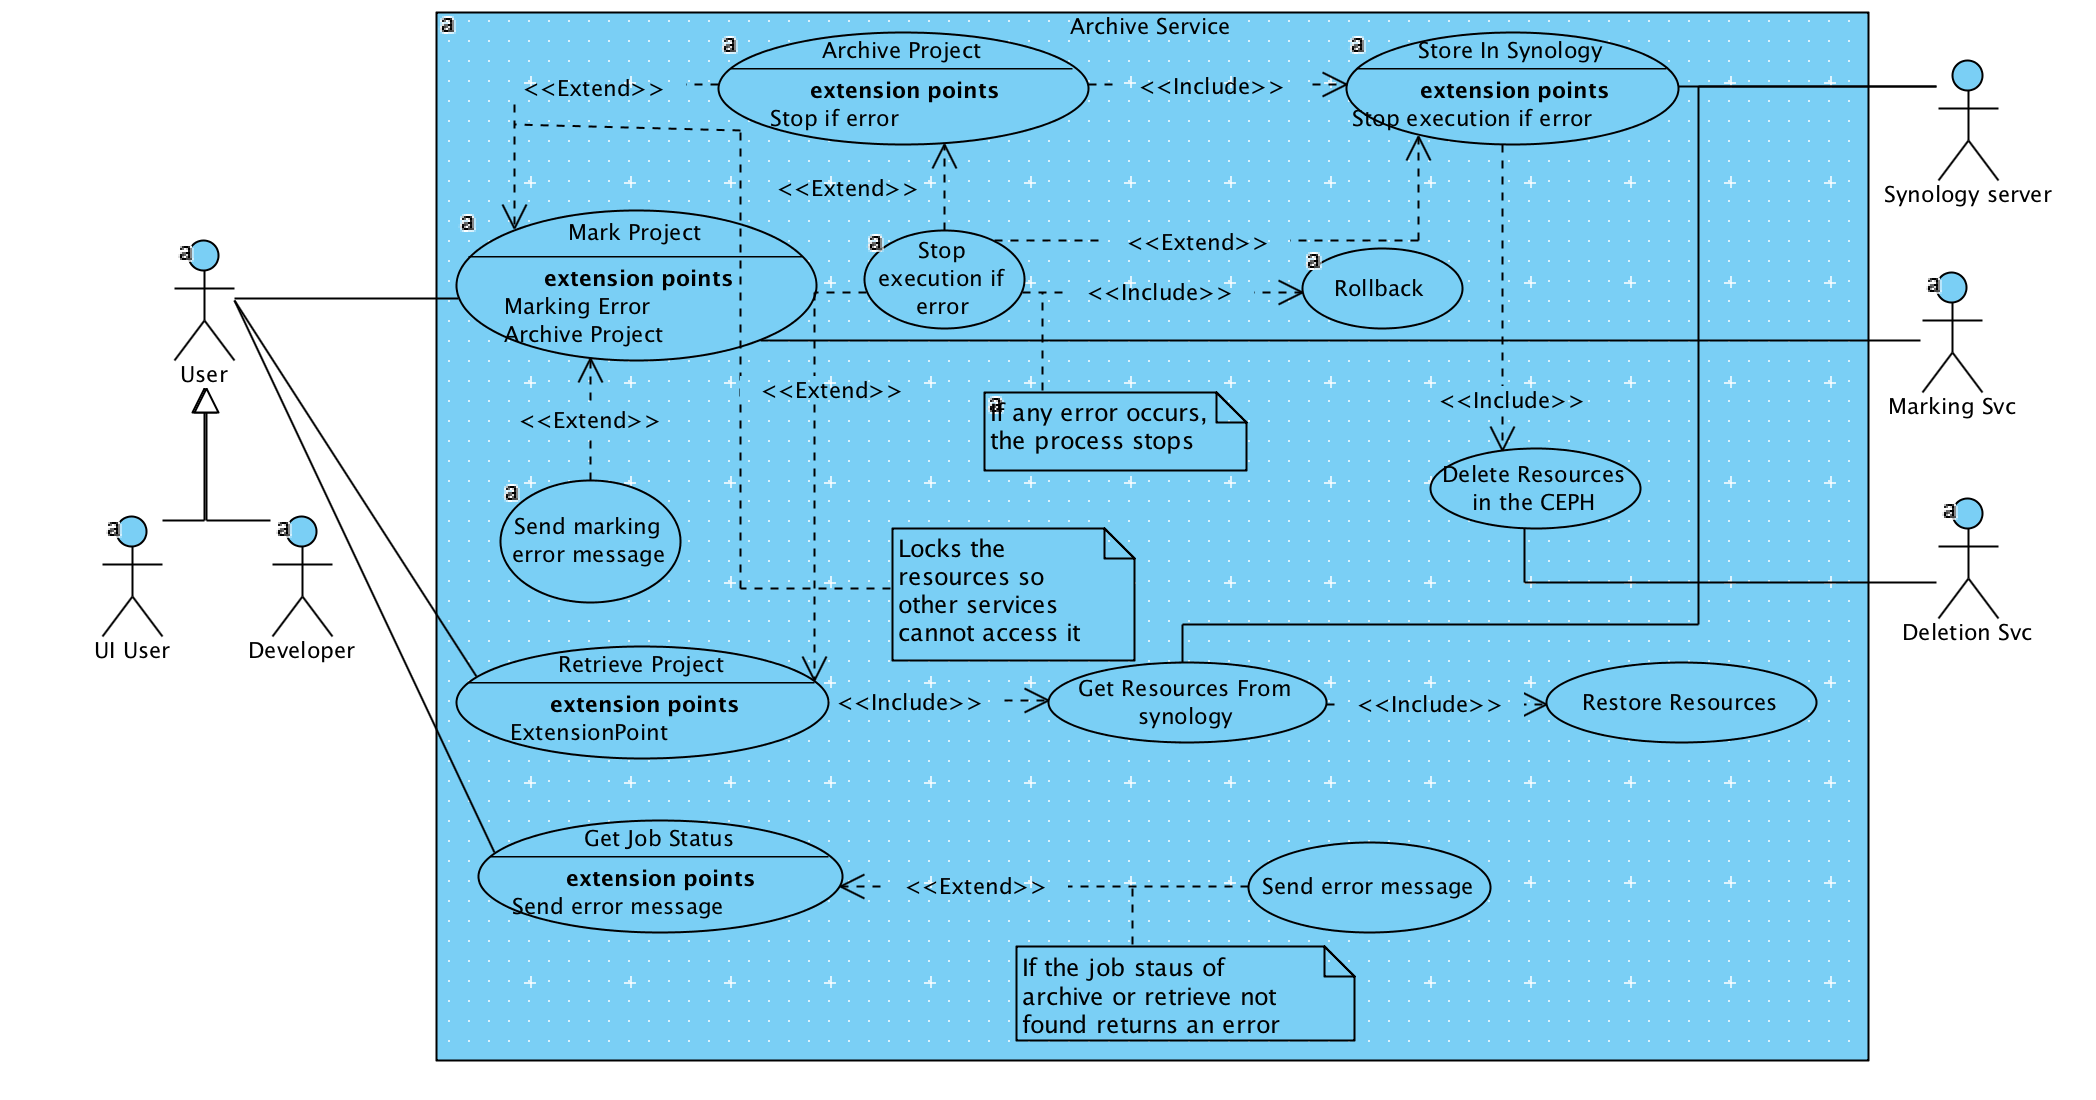
\includegraphics[scale=0.6, angle=90, origin=c]{grafiken/archiveUseCase.png}
    \caption{Use case diagram for Archive service}
    \label{fig:archiveUseCase}
\end{figure}
 